\documentclass[11pt]{article}
\usepackage{naacl2012}
\usepackage{times}
\usepackage{latexsym}
\usepackage{amsmath}
\usepackage{algorithm}
\usepackage{algorithmic}
\usepackage{multirow}
\usepackage{url}
\usepackage{graphicx} 
\usepackage{longtable}
\usepackage{caption}
\usepackage{tipa}

\DeclareMathOperator*{\argmax}{arg\,max}
%\setlength\titlebox{6.5cm}
\setlength\titlebox{2.7cm}

\title{Experiments: Phrase-based MT + Bilingual Lexicon Induction (DRAFT)}
\author{Ann Irvine and Chris Callison-Burch}
\date{\today}

\begin{document}

\maketitle

\section{Introduction}
This preliminary technical report describes three sets of experiments which are related to low resource machine translation. The first set evaluates a bilingual lexicon induction technique and the second two train a phrase-based MT system with scores and translations based on bilingual lexicon induction.

We first evaluate the performance of a Rapp-style \cite{Rapp1999} bilingual lexicon induction framework. We use monolingual web crawl and Wikipedia data to rank candidate translations for a given source language word. We perform experiments identifying English translations for words in 23 source languages. We evaluate our results against dictionaries compiled using Mechanical Turk. 

We then train a phase-based MT system \cite{Moses} with the scores and translations that are the output of our bilingual lexicon induction framework. We use the Mechanical Turk dictionaries, scores based on monolingual data, and induced translations to translate the same five Wikipedia pages for each of our 24 languages of interest. Because bilingual test sets do not exist for every language on our list, we do a qualitative analysis of the machine translation outputs.

In our third set of experiments, we evaluate our techniques in the standard way, by measuring performance with the BLEU metric on bilingual test sets. In these experiments, we vary the amount of bilingual training data that we use to train the model. We also compare systems based only on parallel sentences with those which also access dictionaries and induced translations for OOV unigrams.


%\section{Background}
%\subsection{Phrase-Based SMT}
%\subsection{Low Resource MT}
%\subsection{Lexicon Induction}

\section{Data}
\subsection{Monolingual data}
{\bf Web crawls} We have crawled online news websites for monolingual data in many of the world's languages. We used language-labeled Wikipedia data to train a language classifier. Because our data is comprised of news stories, each document also has an associated time stamp, which is used for calculating temporal similarity (see Section \ref{ssec:temporal}). The amount of data that we have gathered for each of our 24 languages of interest is shown in Table \ref{table:crawls}.

\begin{table}\footnotesize
\begin{center}
\begin{tabular}{|l|c|l|c|}
\hline
Language & word tokens & Language & word tokens \\
\hline
%Malaysian & $57$ & Azeri & $124$ \\
Azeri & $124$k & Nepali & $127$k \\
Tamil & $189$k & Somali & $451$k \\
Uzbek & $627$k & Romanian & $2.9$M \\
Albanian & $3.3$M & Indonesian & $3.8$M \\
Welsh & $3.9$M & Bengali & $4.0$M \\
Serbian & $5.7$M & Bosnian & $7.4$M \\
Polish & $7.8$M & Turkish & $9.1$M \\
Ukrainian & $15.2$M & Bulgarian & $30.5$M \\
Latvian & $35.1$M & Hindi & $42.1$M \\
Slovak & $109$M & Urdu & $285$M \\
Farsi & $698$M & Spanish & $783$M \\
Russian & $1.5$B & &\\
\hline
\end{tabular}
\end{center}
%\vskip -0.1in
\caption{\label{table:crawls}Amount of monolingual online news crawls data, by language.}
%\vskip -0.15in
\end{table}


{\bf Wikipedia} In addition to our data from web crawls, we also use Wikipedia as a source of monolingual data. To maximize the degree of comparability between our source language Wikipedia pages and English Wikipedia, we only use those pages which have interlingual links with English pages. The amount of Wikipedia data that we use for each language is given in Table \ref{table:wiki}.

\begin{table}\footnotesize
\begin{center}
\begin{tabular}{|l|c|l|c|}
\hline
Language & word tokens & Language & word tokens \\
\hline
Azeri & $2.5$M & Nepali & $262$k \\
Tamil & $3.5$M & Somali & $82$k \\
Uzbek & $747$k & Romanian & $21.2$M \\
Albanian & $3.2$M & Indonesian & $18.0$M \\
Welsh & $3.6$M & Bengali & $2.6$M \\
Serbian & $20.1$M & Bosnian & $5.5$M \\
Polish & $96.7$M & Turkish & $22.1$M \\
Ukrainian & $22.4$M & Bulgarian & $19.0$M\\
Latvian & $5.1$M & Hindi & $5.3$M\\
Slovak & $15.3$M & Urdu & $2.2$M\\
Farsi & $12.3$M & Spanish & $189$M\\
Russian & $105$M & &\\
\hline
\end{tabular}
\end{center}
%\vskip -0.1in
\caption{\label{table:wiki}Amount of Wikipedia data, by language.}
%\vskip -0.15in
\end{table}

\subsection {Dictionaries}\label{ssec:dicts}

Throughout the experiments we use two different sets of dictionaries. The first comes from a large collection of dictionaries, gathered from a variety of sources. Some were originally paper dictionaries which were scanned in and digitized with optical character recognition (OCR). Others were originally electronic dictionaries. For some languages, we have multiple dictionaries, and we have simply concatenated them for the experiments described here. Some dictionaries only contain translations of individual words while others contain translations of some source language phrases. In this report, these dictionaries will be referred to as the {\it standard dictionaries}. 

We also use a set of dictionaries that were created using Mechanical Turk. In that dictionary creation, source language words were chosen starting with the most frequent words in that language's Wikipedia \footnote{Is that true?}. Although all of the source words in the Wikipedia dictionaries are unigrams, we allowed workers to translate them into multi-word English phrases. 

Both the standard dictionaries and the MTurk dictionaries are described in Table \ref{table:dicts}.

\begin{table*}\footnotesize
\begin{center}
\begin{tabular}{|l||c|c|c||c|c||c|}
\hline
\multirow{2}{*}{Language} & \multicolumn{3}{|c||}{Standard dictionary} & \multicolumn{2}{|c||}{MTurk dictionary} & \multirow{2}{*}{Script}\\ \cline{2-6}
& Source words &Translations & Dict Source & Source words & Translations & \\
%Language & Src Tokens & Translations & Dict Source(s) \\
\hline
Azeri  & $227,727$ & $231,891$ &  e+o & $7,814$ & $8,121$ & r \\
Nepali  & $4,770$ & $6,812$ &  o & $12,314$ & $17,752$ & d \\
Tamil  & $58,236$ & $165,004$ &   e  & $9,146$ & $14,551$ & o \\
Somali  & $227$ & $230$ &   e & $9,881$ & $11,157$ & r \\
Uzbek  & $124,989$ & $190,688$ & e+o & $5,163$ & $6,710$ & r \\
Romanian  & $48,088$ & $249,479$ &  e & $9,131$ & $12,362$ & r \\
Albanian  & $44,245$ & $188,563$ &  e  & $9,736$ & $12,041$ & r\\
Indonesian  & $32,311$ &  $67,633$ & e+o & $9,236$ & $12,594$ & r\\
Welsh  & $14,586$ &  $25,832$ &   e & $9,013$ & $9,357$ & r\\
Bengali  & $1,481$ & $1,606$   & e & $9,461$ & $14,777$ & o \\
Serbian  &  $55,349$ & $168,140$ & e & $9,622$ & $13,511$ & c, r\\
Bosnian    & $9,641$ & $18,283$ & o & $9,681$ & $13,366$ & r\\
Polish  & $56,233$ &  $261,463$ &   e & $9,467$ &  $13,725$ & r\\
Turkish  & $488,738$ &  $1,272,881$  & e+o & $9,403$ &  $13,686$ & r \\
Ukrainian    & $8,324$ & $14,056$ &  e   & $8,119$ & $8,533$ & c\\
Bulgarian  & $72,720$ & $316,631$ &  e  & $9,607$ &  $12,442$ & c \\
Latvian  & $33,486$ & $148,363$ &   e & $8,624$ &  $9,896$ & r \\
Hindi  & $25,305$ & $58,179$ &   e & $8,014$ & $10,721$ & d\\
Slovak  & $48,683$ & $233,093$   & e  & $9,495$ & $11,998$ & r \\
Urdu  & $24,271$ &  $113,911$  & e & $8,088$ & $11,254$ & a \\
Farsi  & $101,620$ &  $198,605$  &  e+o & $1,845$ & $1,970$ & a \\
Spanish  &  $73,589$  & $347,441$ & e  & $8,970$ & $11,566$ & r \\
Russian  & $89,785$ & $423,009$ & e & $9,188$ & $11,785$ & c \\
\hline
\end{tabular}
\end{center}
%\vskip -0.1in
\caption{\label{table:dicts}Description of both standard and MTurk dictionaries. The number of unique source words and phrases in each dictionary is given along with the total number of translations. The source(s) of each standard dictionary is also given. {\it e} indicates that a dictionary was originally electronic and {\it o} indicates a paper dictionary that was OCR'd. In some cases, we have both types of dictionaries for a given language. The final column indicates whether the primary script used in our dictionaries (as well as monolingual datasets) is Roman (r), Cyrillic (c), Arabic (a), Devanagari (d), or other (o).}
%\vskip -0.15in
\end{table*}

\subsection{Languages}
We selected the 23 languages because, for each, we had access to standard and MTurk dictionaries as well as some monolingual data from both the web crawls and Wikipedia. Additionally, we included some truly low resource languages (e.g. Somali, Nepali) and also some high resource languages for which we could more thoroughly evaluate MT performance (e.g. Urdu, Spanish).

\section{Experiments 1: Bilingual lexicon induction}\label{sec:lexinduc}
In our first set of experiments, we evaluate the quality of a bilingual lexicon induction framework that combines monolingual distributional, temporal, and orthographic signals to rank target language word translations for a given source language unigram. 

\subsection{Contextual Similarity} 
We score monolingual distributional similarity by first collecting contextual vectors for each source and target language word. The contextual vector for a given source language word, $w_{s_i}$, is the size of the source language vocabulary, $|V_s|$, and contains counts of how many times each word in the source language vocabulary appeared in the context of word $w_{s_i}$. In the experiments presented here, we use bag of words contexts in a window of size two (two words to the left of $w_{s_i}$ and two words to the right). Similarly, we collect context vectors for all target language words, $w_{t_j}$. In all experiments, we use both the standard dictionaries and the MTurk dictionaries to project the target language contextual vectors into the source language feature space.% in order to keep the dictionary size and quality constant across all source languages. 
We gather both source and target language contextual vectors from our web crawl data.

\subsection{Temporal Similarity}\label{ssec:temporal}
We gather temporal signatures for each source and target language unigram from our time-stamped web crawl data. That is, temporal signatures for a given word contain counts corresponding to how many times that word appeared in news articles with a certain date. We expect that source and target language words which are translations of one another will appear with similar frequencies over time in monolingual data. We collect temporal signatures over dates for which we have monolingual data in both languages. Our English web crawl data is essentially limitless, so we restrict the English data that we use in a particular source language experiment to be no more than three times the size of our source language web crawled data, and only include news articles from those dates for which we also have source language articles. In all experiments in this report, we use a sliding window of three days to estimate temporal similarity between a pair of word or phrase temporal signatures.

\subsection{Orthographic Similarity} 
We measure orthographic similarity between a pair of words as the normalized\footnote{Normalized by the average of the lengths of the two words} edit distance between the two words. For non-roman script languages, we transliterate words into the roman script before measuring orthographic similarity. For word classes that tend to be transliterated, rather than translated, (e.g. person and place names), we expect the edit distances between English words and their translations to be small. 

\subsection{Score Aggregation} 
Rather than using absolute scores, we aggregate the {\it ranked lists} provided by each of the above three similarity measures. That is, for a given source language word, we score and rank all target language candidate translations (the target language vocabulary) using each of the above three metrics. We then compute the {\it mean reciprocal rank} (MRR) for each target language word and produce a new ranking based on the MRRs.

\subsection{Results}

%{\bf Quantitative} 

For each source language, we evaluate the above bilingual lexicon induction framework using percent accuracy in the top-1, top-10, and top-100 ranked target language word lists, compared against the MTurk dictionaries. This measure is somewhat conservative since the MTurk dictionaries aren't expected to be exhaustive, meaning that some target language translations for a given source language word won't appear in the dictionary and the system won't be given credit for ranking these target items high in its translation list. We use the MTurk dictionaries only as a gold standard in order to keep the dictionary size and quality constant across all source languages. For each source language word, the target language list of candidate translations contains all unique word types observed in our target language monolingual corpus (in the case of these experiments, English web crawl data). 

Figures \ref{fig:bli.az} through \ref{fig:bli.fa} present the bilingual lexicon induction experimental results. In each experiment, the $3,000$ most frequent source language words in the MTurk dictionary, with respect to the monolingual crawls data, were divided into 10 bins, by frequency. That is, the most frequent 300 source language words were put in the first bin, and the least frequent (among the most frequent 3000) 300 source language words were put into the tenth bin. The horizontal access in each figure plots the average corpus frequency of the words in a given bin versus the percent of those 300 source language words that have a correct translation in the top-k ranked list of translations. In general, our monolingual signals are stronger for those words that appear frequently in monolingual corpora than for those words that appear less frequently and have sparse context and temporal counts. Therefore, translation accuracy tends to be higher for frequent words than for less frequent words, resulting in accuracies that go up from left to right, or from lower frequency to higher frequency, in the figures.
 
The results are presented starting with the language with the least amount of monolingual web crawl data (Azeri, Figure \ref{fig:bli.az}) and ending with the language with the largest amount of monolingual web crawl data (Farsi, Figure \ref{fig:bli.fa}), among those languages for which results are presented. Corpus frequencies for even the most frequent words in the first few source languages are very small. For example, the average frequency of the 300 most frequent Azeri and Nepali words is around 200. For those languages which we have very little monolingual data, all of the contextual and temporal vectors are sparse and, in general, translation accuracies are low.

As we have access to more monolingual data, the figures look more regular. That is, given a sufficient amount of monolingual text, we do observe that our translation accuracy is higher for more frequent source language words than for less frequent source language words. This trend is particularly clear in the Albanian (Figure \ref{fig:bli.sq}) and Indonesian (Figure \ref{fig:bli.id}) plots.

Performance among Indian languages, including Nepali, Hindi, Bengali, and Tamil, is particularly low. While we have collected very small amounts of Nepali and Tamil web crawl monolingual data, the amount of Bengali data is modest, and we have a large amount of Hindi data. Yet, top-100 accuracy for even the most frequent Hindi words is only around 15\%. It is also possible that English and Indian language news articles are less comparable than other language pairs. 

Figure \ref{fig:across-lang-lexinduc} plots the average top-100 accuracy for word bins with an average monolingual corpus frequency of 200 versus the amount of monolingual web crawl data for each of the twenty languages explored in this section. {\it Within a set of related languages}, an increase in monolingual data improves accuracy in some cases. For example, performance on Slovak and Bulgarian is higher than that of Serbian and Ukrainian, and have access to more monolingual data for those languages. Across all languages, however, this correlation isn't consistent. For example, performance on Somali is very good despite the limited amount of monolingual data.


%{\bf Qualitative} 
%Table \ref{table:lexinducexamples} shows lists of ranked translations under each of our similarity metrics for several words in each of our source languages.



\begin{figure}[h]
%\vskip 0.0in
\begin{center}
\includegraphics[width=0.9 \linewidth]{../byFreqGraphs/az/lexinductnew.pdf}
\vskip -0.15in
\caption{Azeri bilingual lexicon induction results}
%\vskip -0.2in
\label{fig:bli.az} 
\end{center}
\end{figure}

\begin{figure}[h]
%\vskip 0.0in
\begin{center}
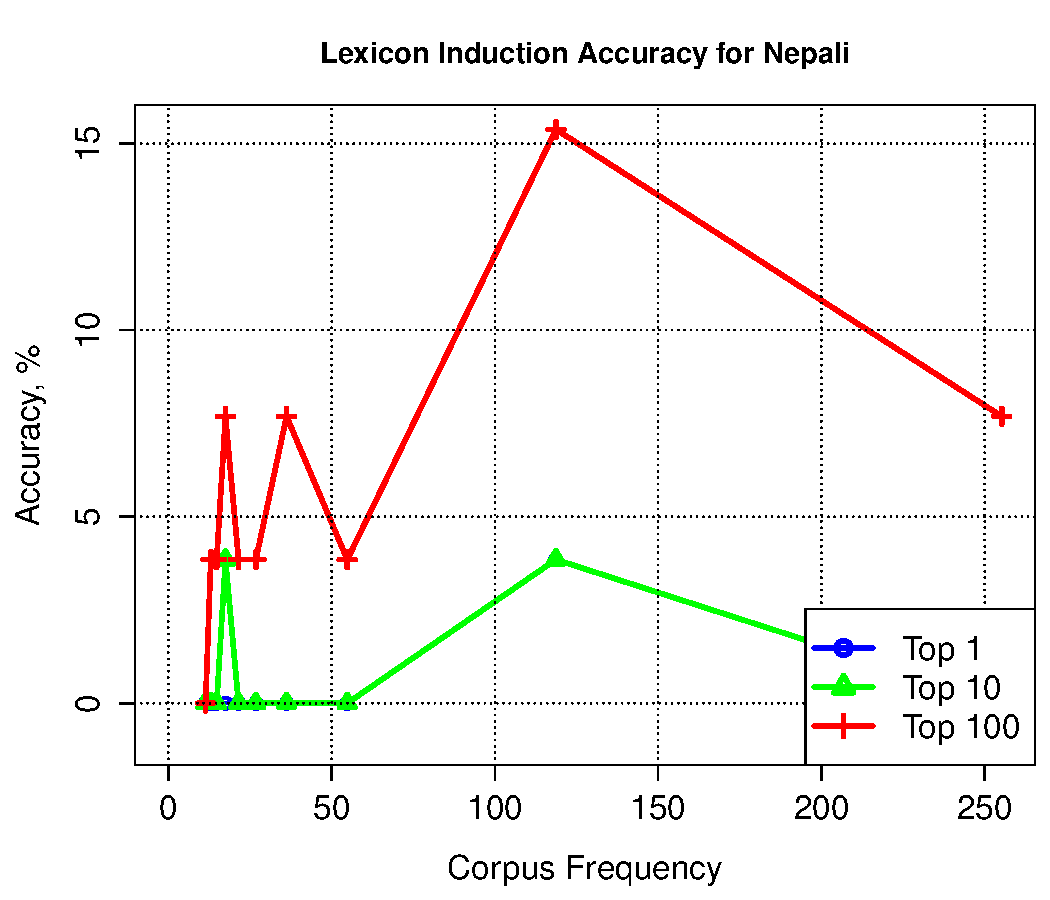
\includegraphics[width=0.9 \linewidth]{../byFreqGraphs/ne/lexinductnew.pdf}
\vskip -0.15in
\caption{Nepali bilingual lexicon induction results}
%\vskip -0.2in
\label{fig:bli.ne} 
\end{center}
\end{figure}

\begin{figure}
%\vskip 0.0in
\begin{center}
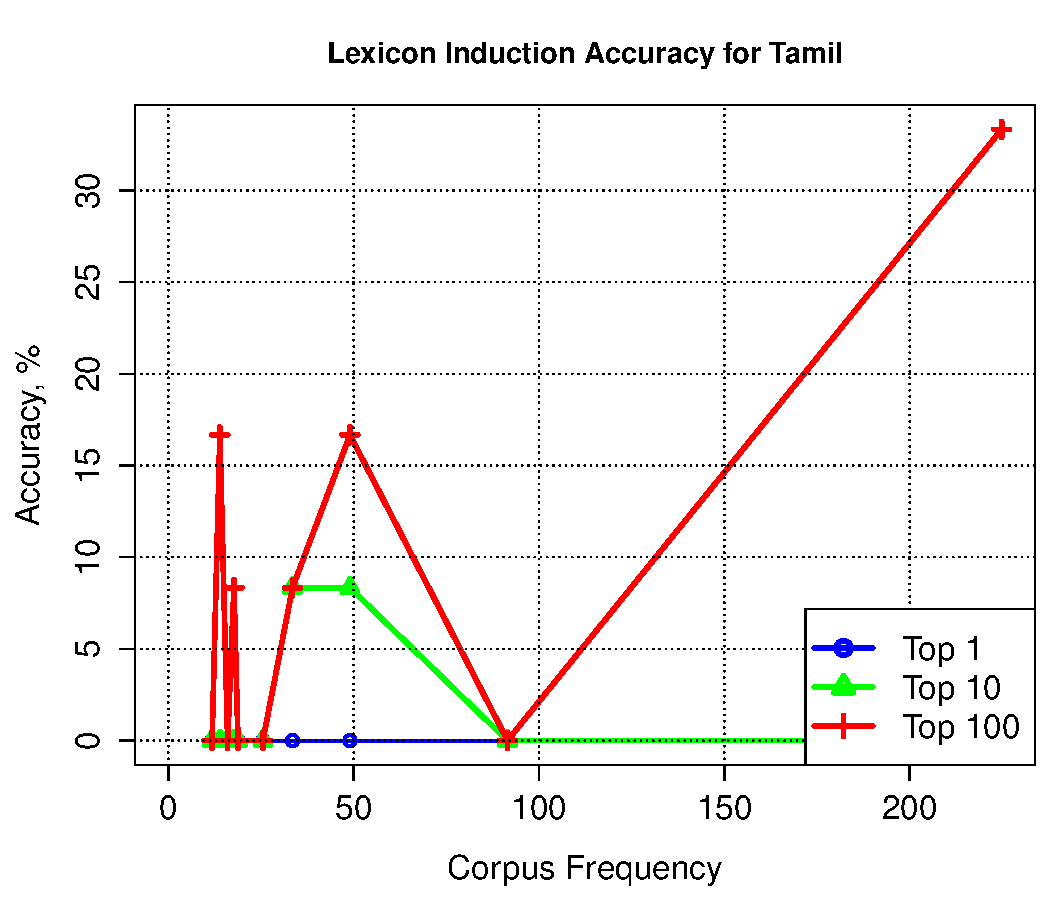
\includegraphics[width=0.9 \linewidth]{../byFreqGraphs/ta/lexinductnew.pdf}
\vskip -0.15in
\caption{Tamil bilingual lexicon induction results}
%\vskip -0.2in
\label{fig:bli.ta} 
\end{center}
\end{figure}

\begin{figure}
%\vskip 0.0in
\begin{center}
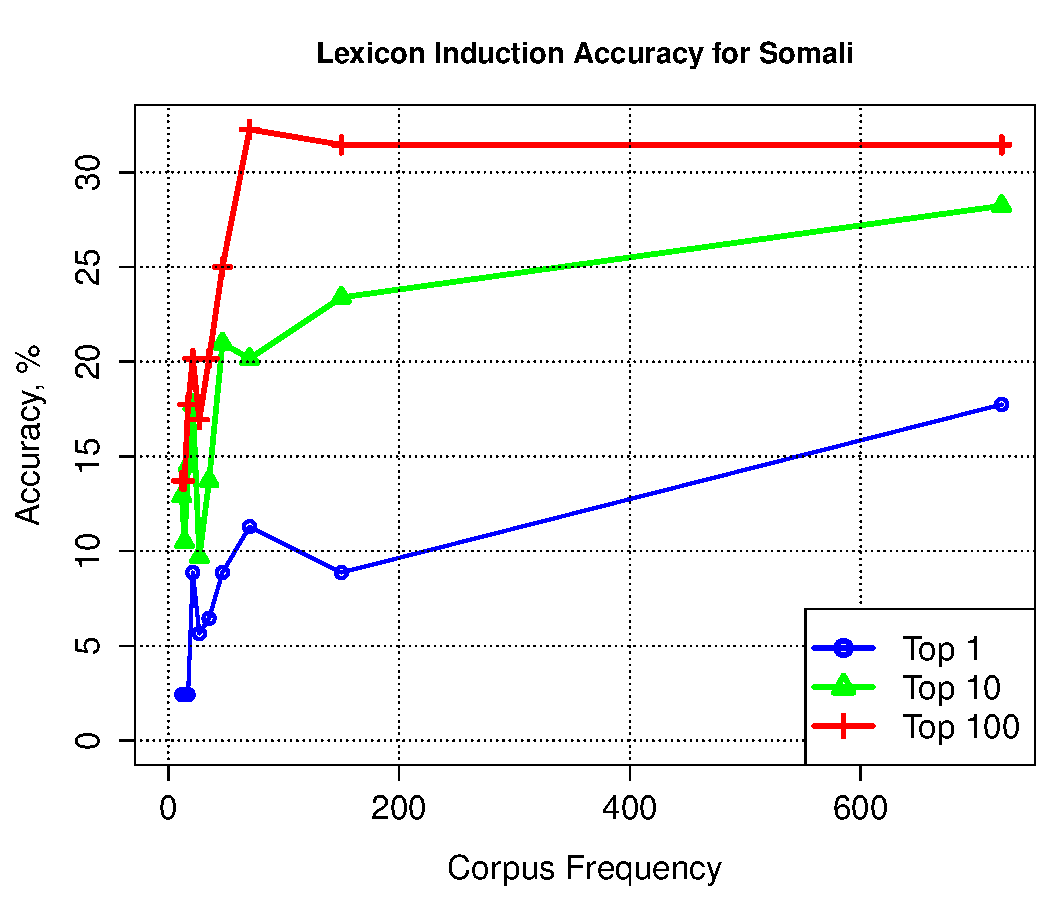
\includegraphics[width=0.9 \linewidth]{../byFreqGraphs/so/lexinductnew.pdf}
\vskip -0.15in
\caption{Somali bilingual lexicon induction results}
%\vskip -0.2in
\label{fig:bli.so} 
\end{center}
\end{figure}

\begin{figure}
%\vskip 0.0in
\begin{center}
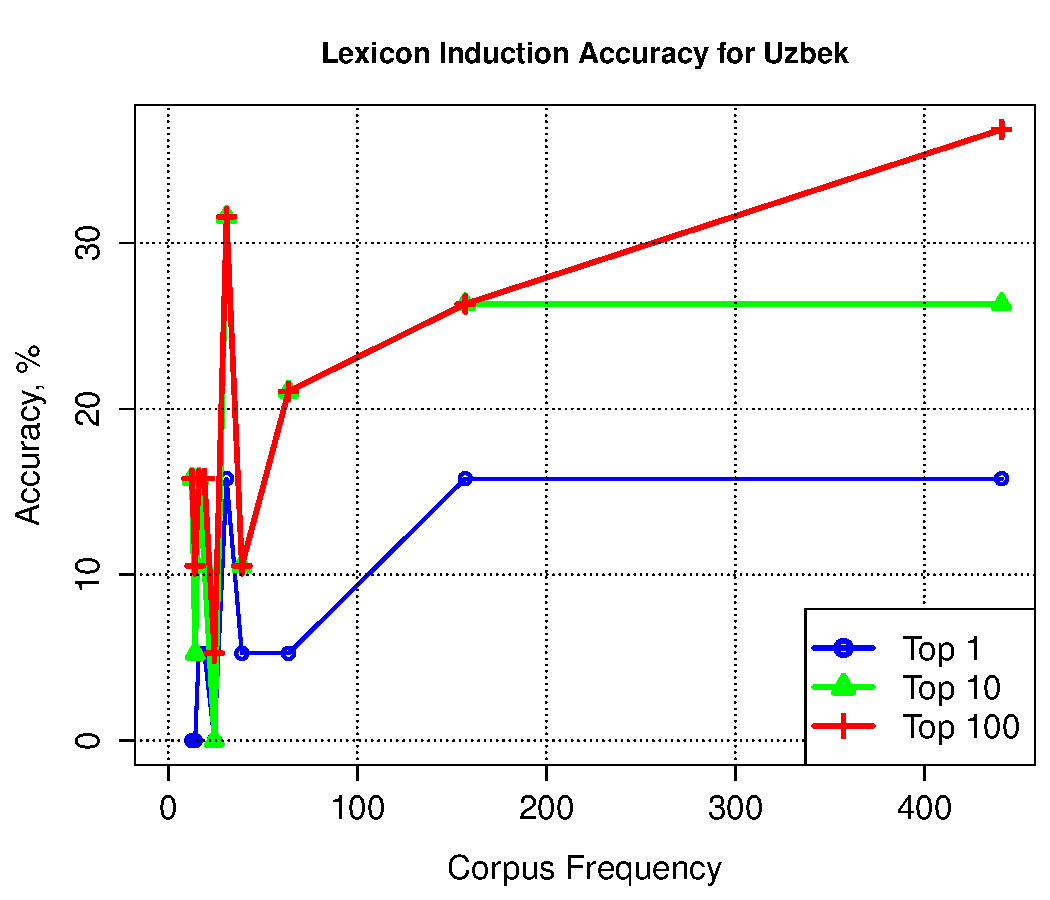
\includegraphics[width=0.9 \linewidth]{../byFreqGraphs/uz/lexinductnew.pdf}
\vskip -0.15in
\caption{Uzbek bilingual lexicon induction results}
%\vskip -0.2in
\label{fig:bli.uz} 
\end{center}
\end{figure}

\begin{figure}
%\vskip 0.0in
\begin{center}
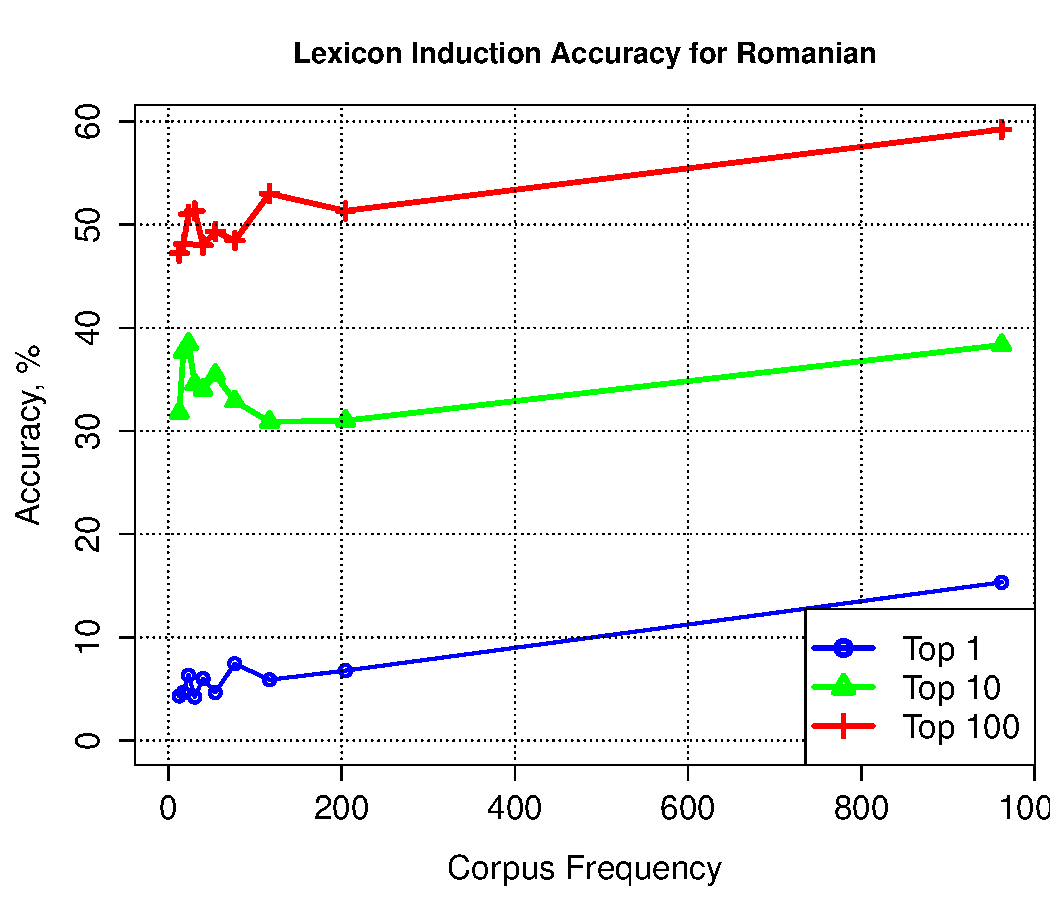
\includegraphics[width=0.9 \linewidth]{../byFreqGraphs/ro/lexinductnew.pdf}
\vskip -0.15in
\caption{Romanian bilingual lexicon induction results}
%\vskip -0.2in
\label{fig:bli.ro} 
\end{center}
\end{figure}



\begin{figure}
%\vskip 0.0in
\begin{center}
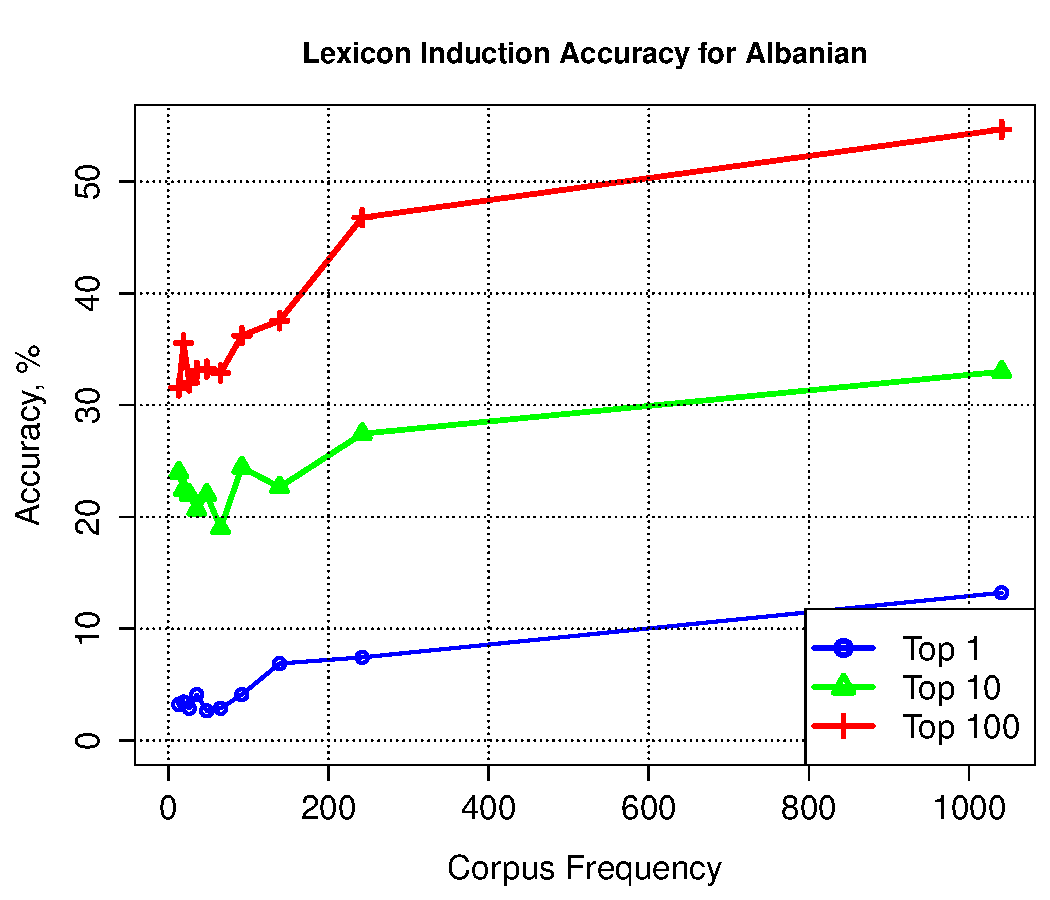
\includegraphics[width=0.9 \linewidth]{../byFreqGraphs/sq/lexinductnew.pdf}
\vskip -0.15in
\caption{Albanian bilingual lexicon induction results}
%\vskip -0.2in
\label{fig:bli.sq} 
\end{center}
\end{figure}

\begin{figure}
%\vskip 0.0in
\begin{center}
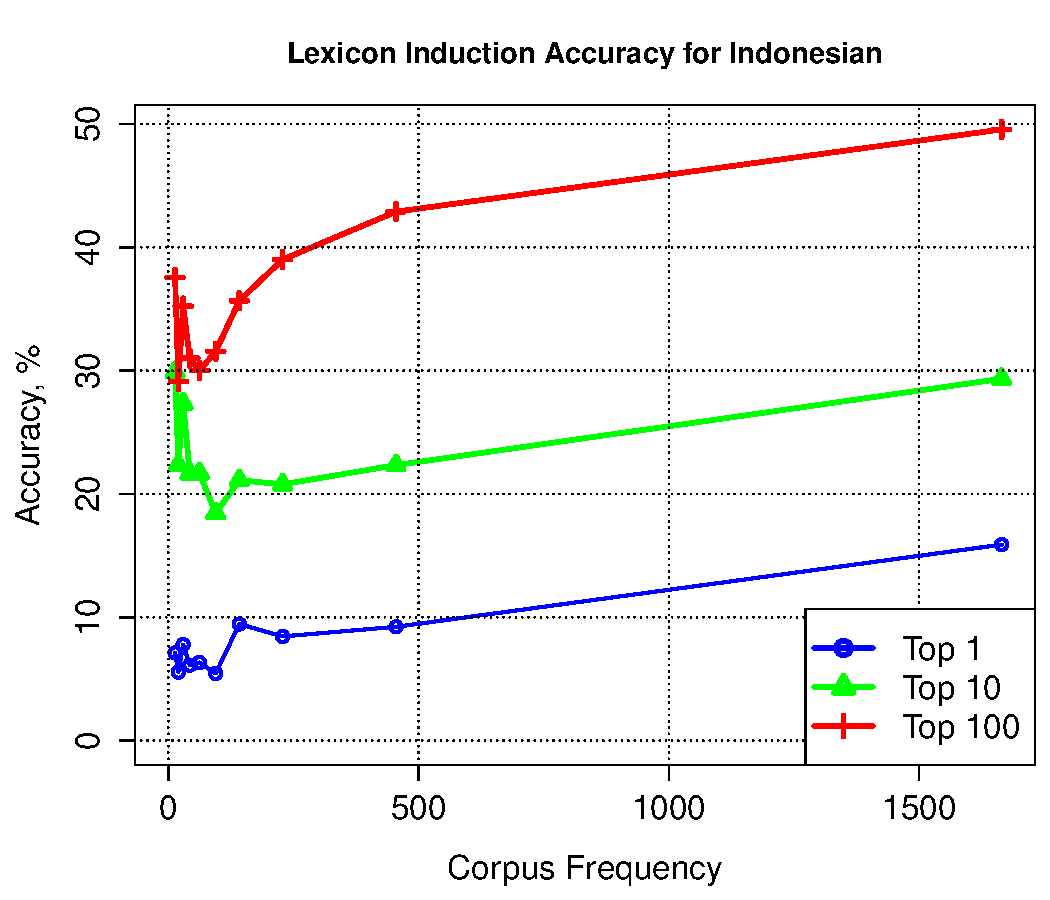
\includegraphics[width=0.9 \linewidth]{../byFreqGraphs/id/lexinductnew.pdf}
\vskip -0.15in
\caption{Indonesian bilingual lexicon induction results}
%\vskip -0.2in
\label{fig:bli.id} 
\end{center}
\end{figure}



\begin{figure}
%\vskip 0.0in
\begin{center}
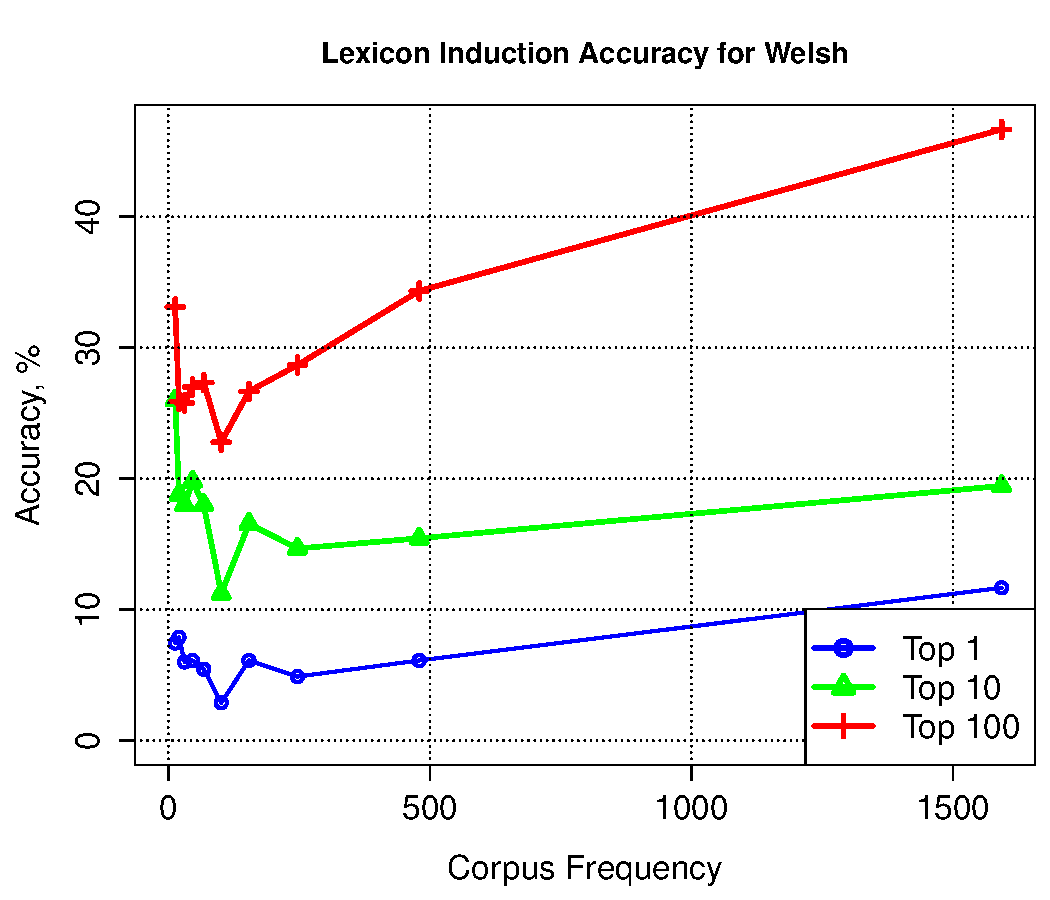
\includegraphics[width=0.9 \linewidth]{../byFreqGraphs/cy/lexinductnew.pdf}
\vskip -0.15in
\caption{Welsh bilingual lexicon induction results}
%\vskip -0.2in
\label{fig:bli.cy} 
\end{center}
\end{figure}



\begin{figure}
%\vskip 0.0in
\begin{center}
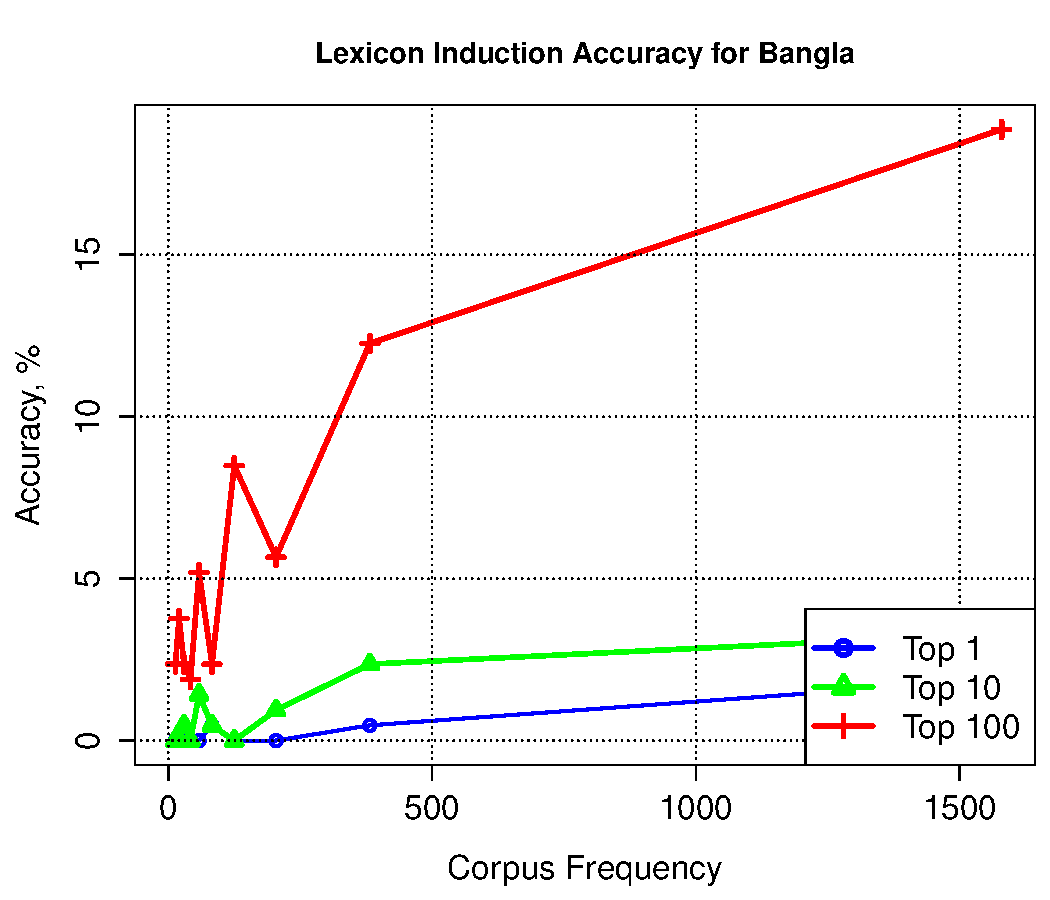
\includegraphics[width=0.9 \linewidth]{../byFreqGraphs/bn/lexinductnew.pdf}
\vskip -0.15in
\caption{Bengali bilingual lexicon induction results}
%\vskip -0.2in
\label{fig:bli.bn} 
\end{center}
\end{figure}

\begin{figure}
%\vskip 0.0in
\begin{center}
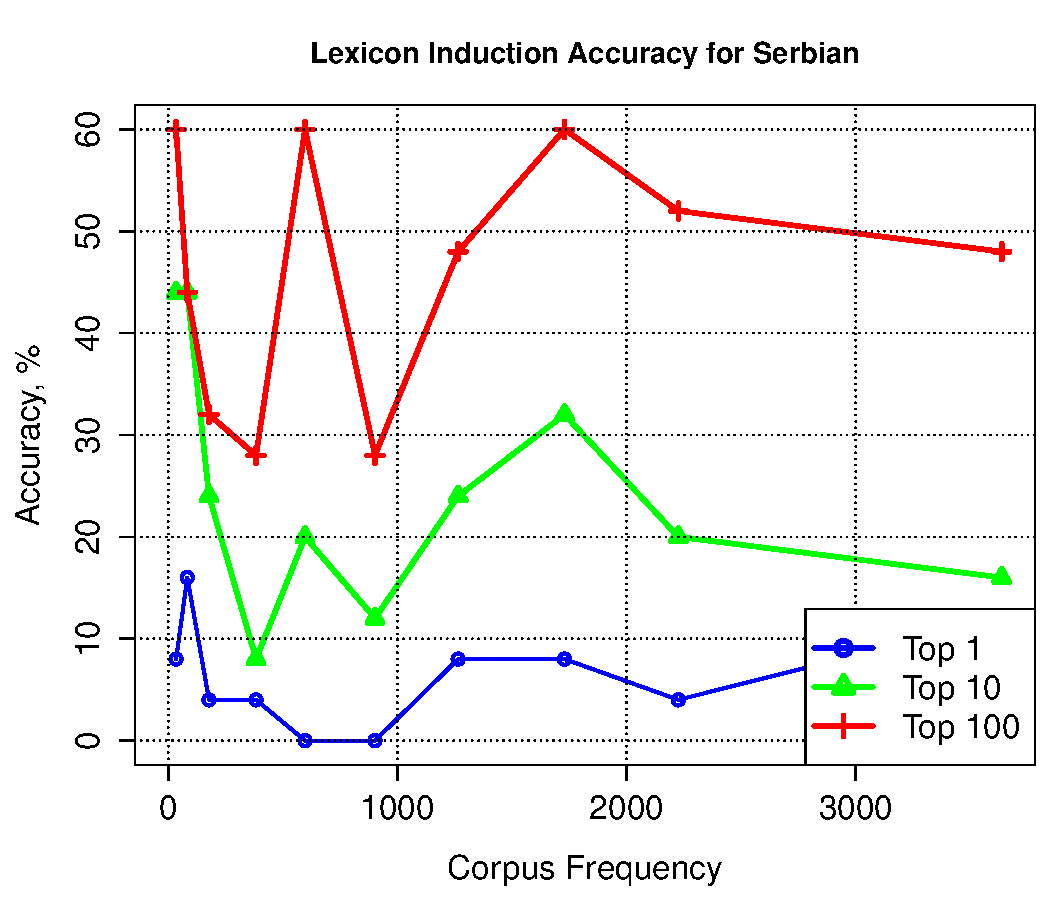
\includegraphics[width=0.9 \linewidth]{../byFreqGraphs/sr/lexinductnew.pdf}
\vskip -0.15in
\caption{Serbian bilingual lexicon induction results}
%\vskip -0.2in
\label{fig:bli.sr} 
\end{center}
\end{figure}


\begin{figure}
%\vskip 0.0in
\begin{center}
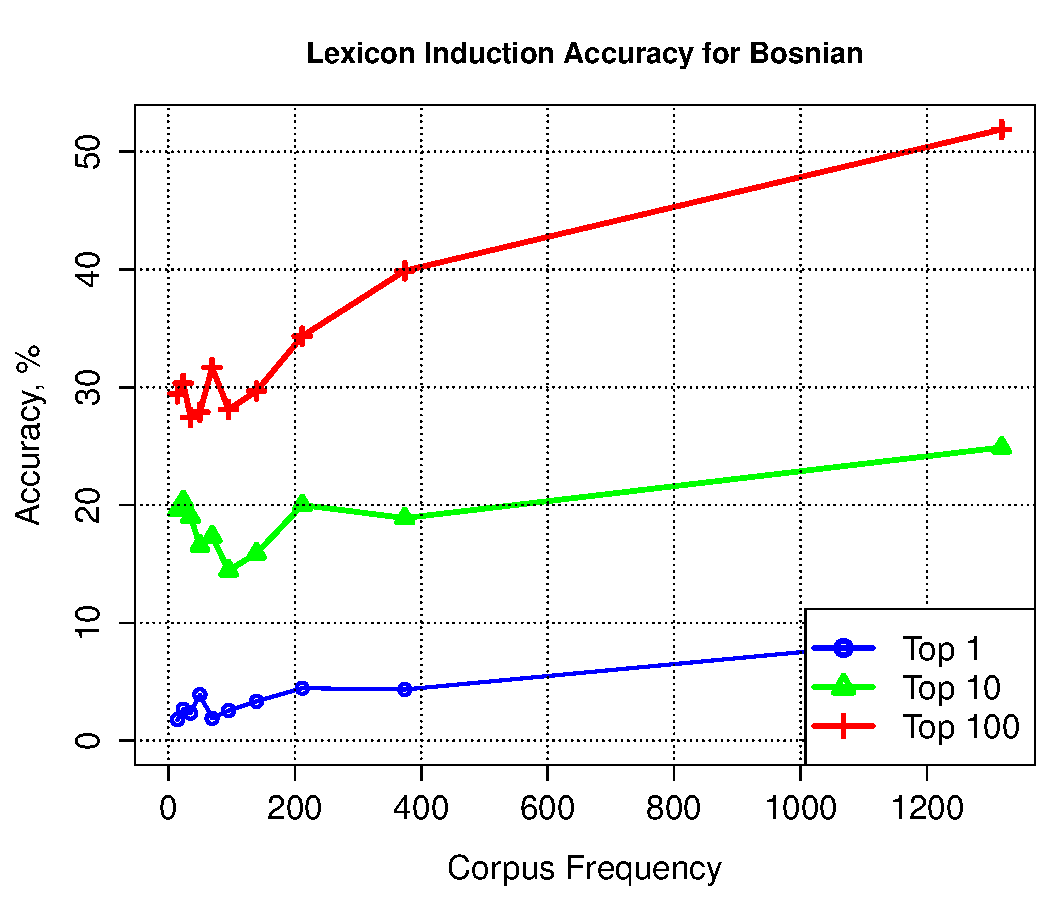
\includegraphics[width=0.9 \linewidth]{../byFreqGraphs/bs/lexinductnew.pdf}
\vskip -0.15in
\caption{Bosnian bilingual lexicon induction results}
%\vskip -0.2in
\label{fig:bli.bs} 
\end{center}
\end{figure}



\begin{figure}
%\vskip 0.0in
\begin{center}
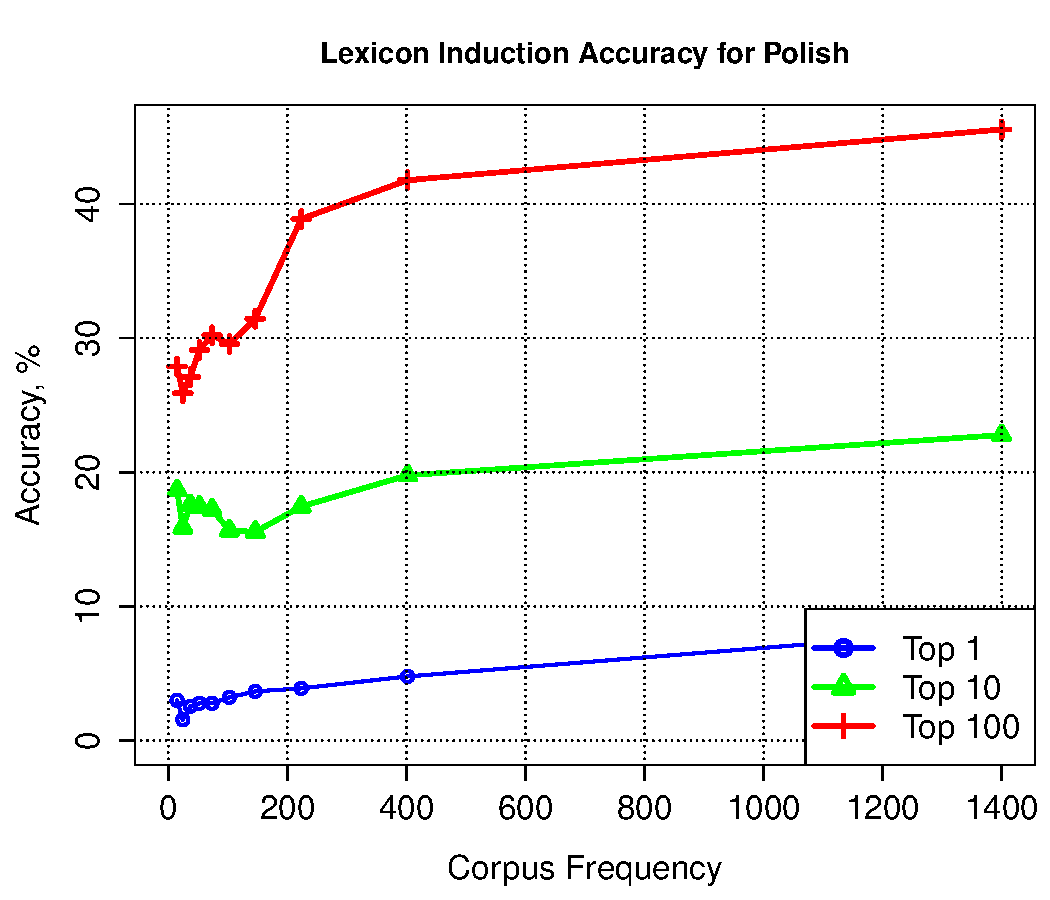
\includegraphics[width=0.9 \linewidth]{../byFreqGraphs/pl/lexinductnew.pdf}
\vskip -0.15in
\caption{Polish bilingual lexicon induction results}
%\vskip -0.2in
\label{fig:bli.pl} 
\end{center}
\end{figure}

\begin{figure}
%\vskip 0.0in
\begin{center}
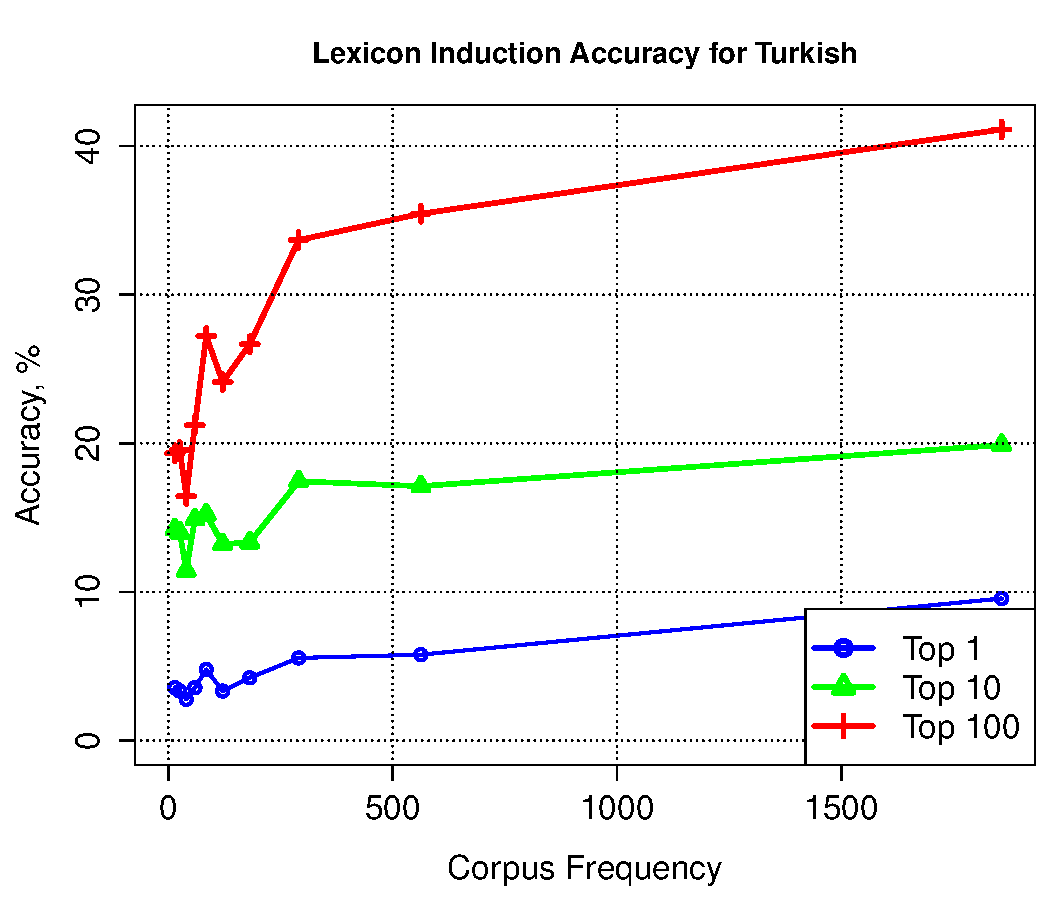
\includegraphics[width=0.9 \linewidth]{../byFreqGraphs/tr/lexinductnew.pdf}
\vskip -0.15in
\caption{Turkish bilingual lexicon induction results}
%\vskip -0.2in
\label{fig:bli.tr} 
\end{center}
\end{figure}



\begin{figure}
%\vskip 0.0in
\begin{center}
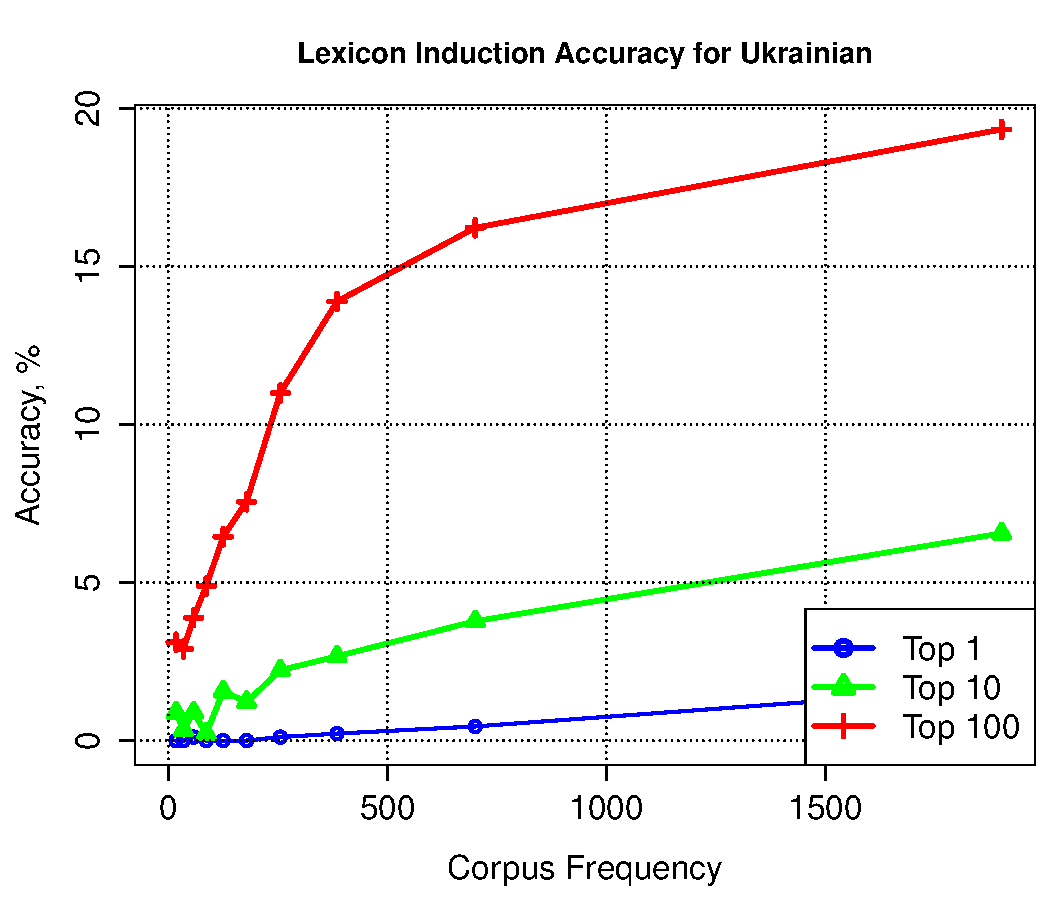
\includegraphics[width=0.9 \linewidth]{../byFreqGraphs/uk/lexinductnew.pdf}
\vskip -0.15in
\caption{Ukrainian bilingual lexicon induction results}
%\vskip -0.2in
\label{fig:bli.uk} 
\end{center}
\end{figure}


\begin{figure}
%\vskip 0.0in
\begin{center}
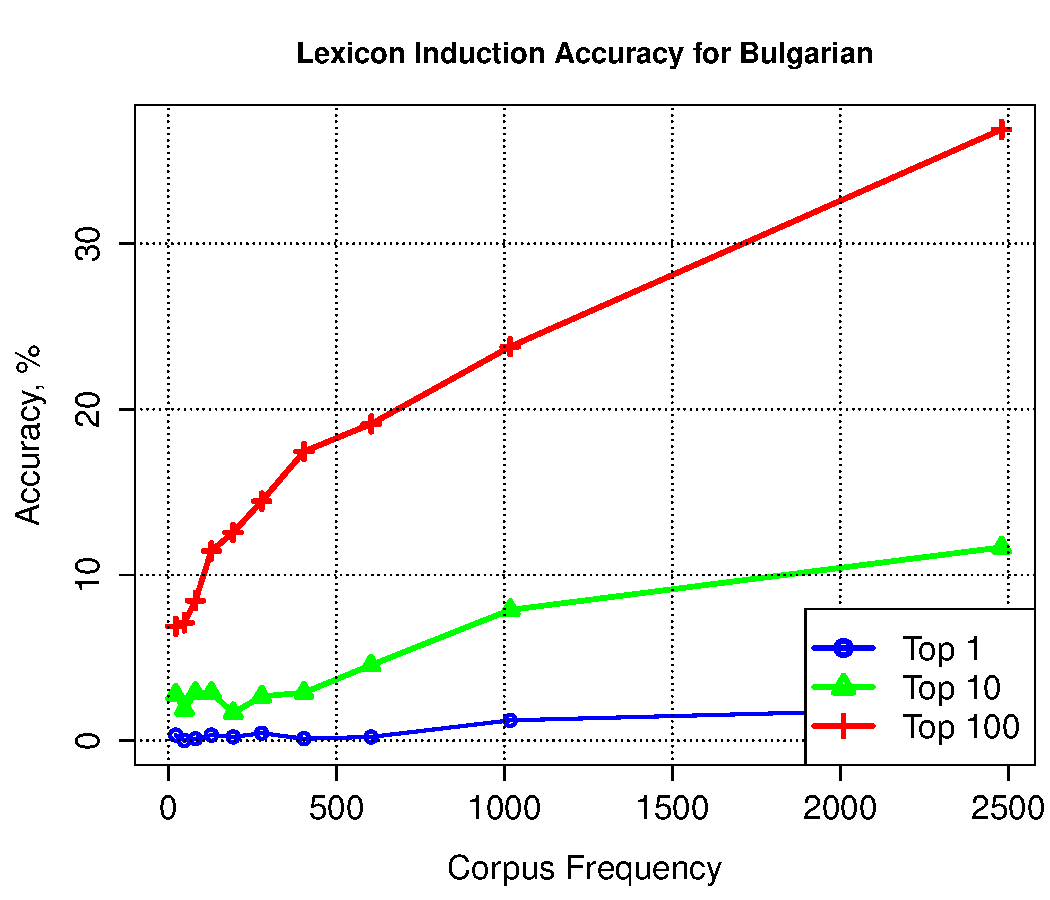
\includegraphics[width=0.9 \linewidth]{../byFreqGraphs/bg/lexinductnew.pdf}
\vskip -0.15in
\caption{Bulgarian bilingual lexicon induction results}
%\vskip -0.2in
\label{fig:bli.bg} 
\end{center}
\end{figure}



\begin{figure}
%\vskip 0.0in
\begin{center}
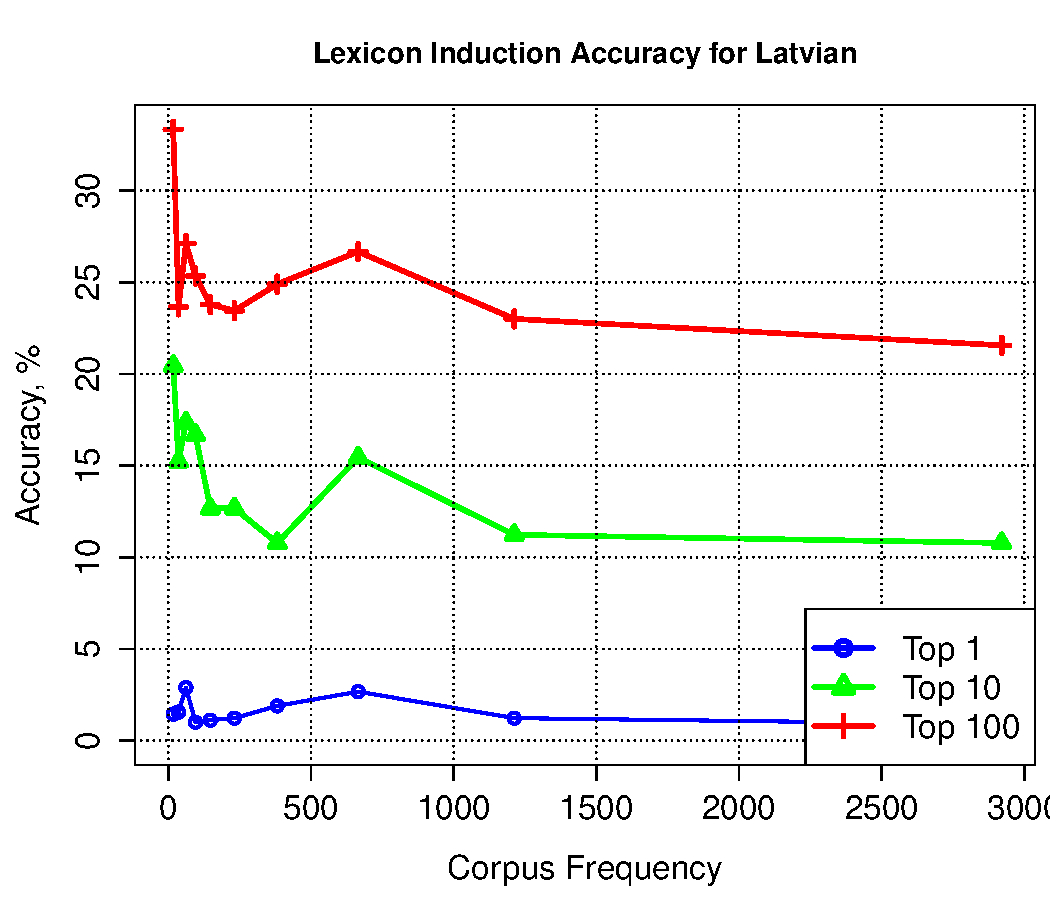
\includegraphics[width=0.9 \linewidth]{../byFreqGraphs/lv/lexinductnew.pdf}
\vskip -0.15in
\caption{Latvian bilingual lexicon induction results}
%\vskip -0.2in
\label{fig:bli.lv} 
\end{center}
\end{figure}

\clearpage


\begin{figure}
\vskip 0.0in
\begin{center}
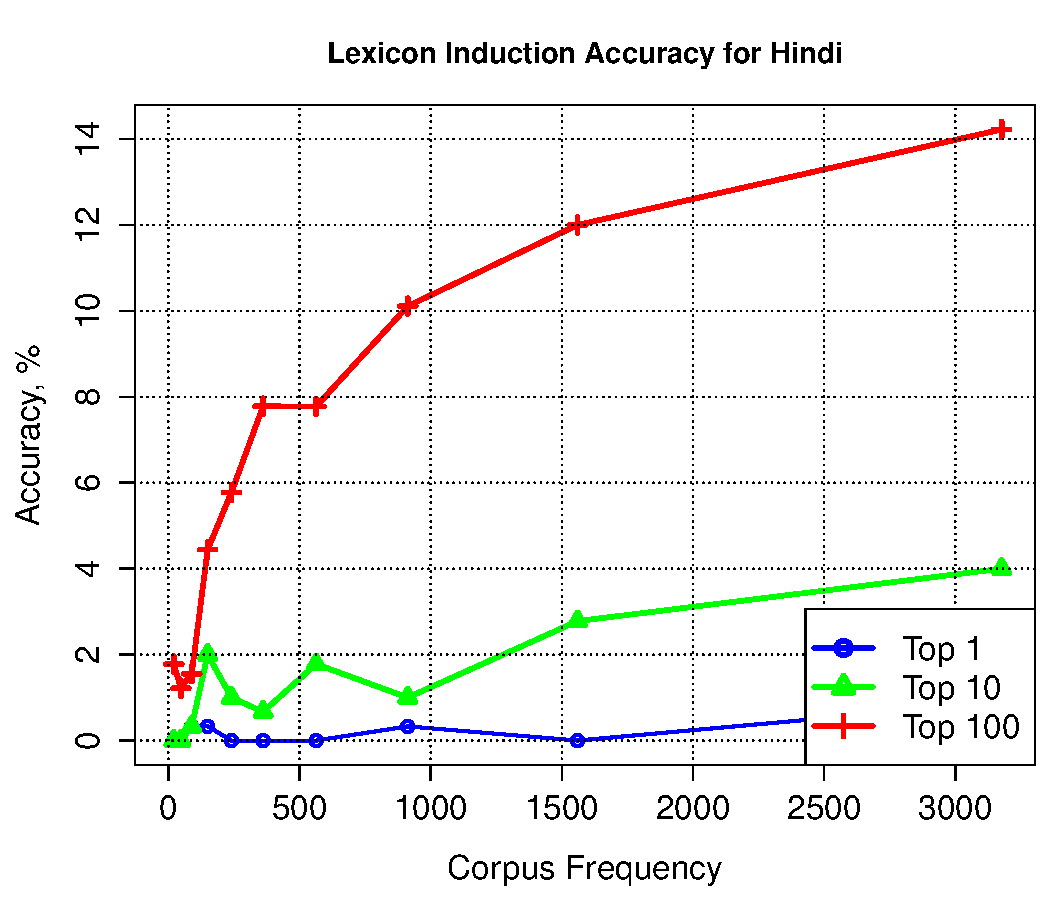
\includegraphics[width=0.9 \linewidth]{../byFreqGraphs/hi/lexinductnew.pdf}
\vskip -0.15in
\caption{Hindi bilingual lexicon induction results}
\vskip -0.2in
\label{fig:bli.hi} 
\end{center}
\end{figure}



\begin{figure}
\vskip 0.0in
\begin{center}
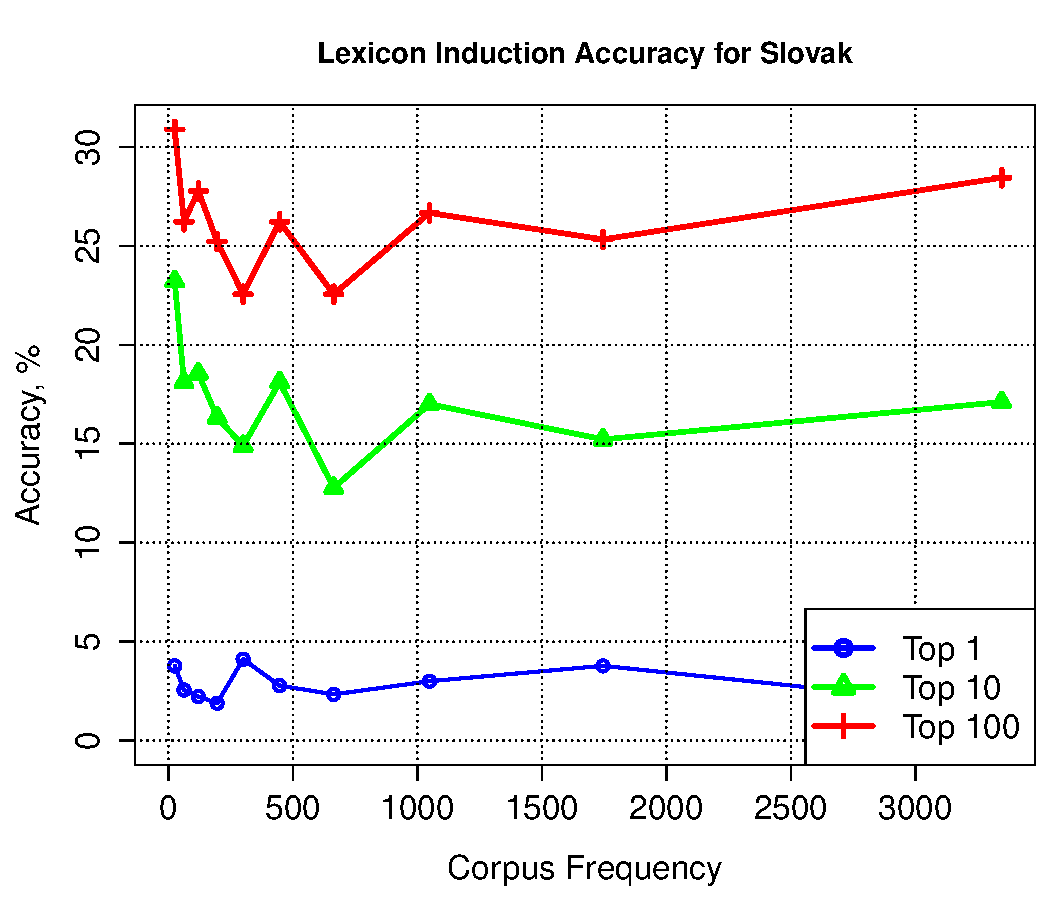
\includegraphics[width=0.9 \linewidth]{../byFreqGraphs/sk/lexinductnew.pdf}
\vskip -0.15in
\caption{Slovak bilingual lexicon induction results}
\vskip -0.2in
\label{fig:bli.sk} 
\end{center}
\end{figure}

\begin{figure}
\vskip 0.0in
\begin{center}
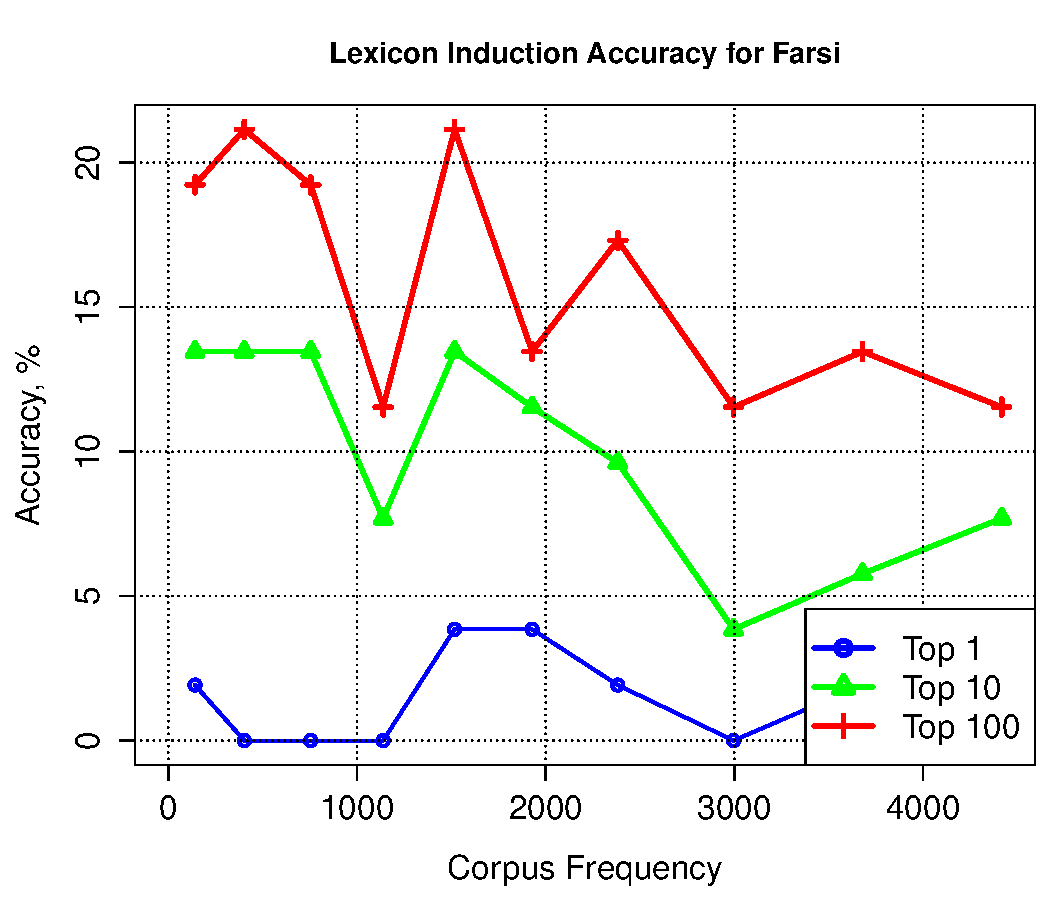
\includegraphics[width=0.9 \linewidth]{../byFreqGraphs/fa/lexinductnew.pdf}
\vskip -0.15in
\caption{Farsi bilingual lexicon induction results}
\vskip -0.2in
\label{fig:bli.fa} 
\end{center}
\end{figure}


\begin{figure}
\vskip 0.0in
\begin{center}
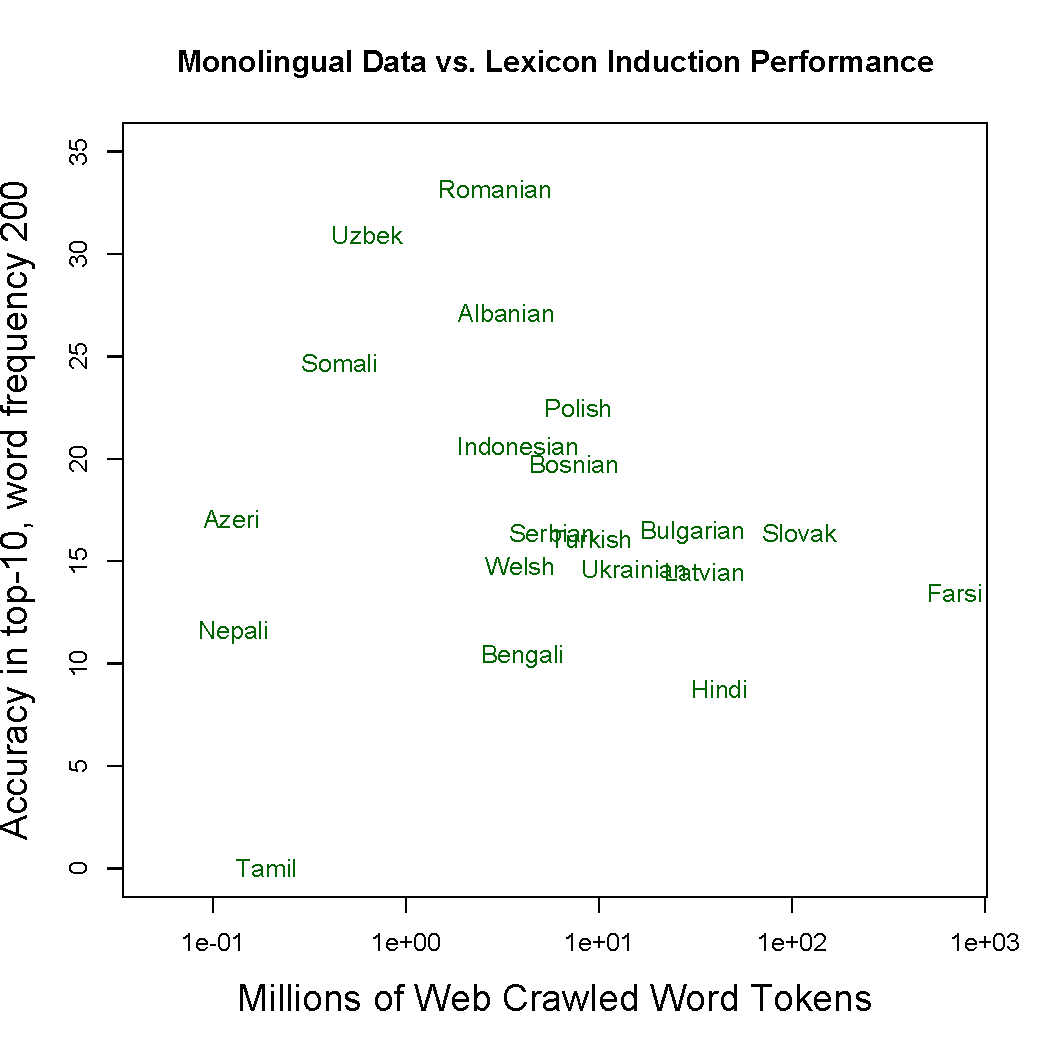
\includegraphics[width=1.1 \linewidth]{../byFreqGraphs/monodatascatter/scatter200.pdf}
\vskip -0.15in
\caption{Monolingual data vs. lexicon induction accuracy}
\vskip -0.2in
\label{fig:across-lang-lexinduc} 
\end{center}
\end{figure}


%\begin{figure}
%\vskip 0.0in
%\begin{center}
%\includegraphics[width=0.9 \linewidth]{/Users/anni/Projects/unsup_translation/babelClean/LIMTresults/byFreqGraphs/ms/lexinductnew.pdf}
%\vskip -0.15in
%\caption{Malaysian bilingual lexicon induction results}
%\vskip -0.2in
%\label{fig:bli.ms} 
%\end{center}
%\end{figure}


%\newpage
%\clearpage


%\begin{table*}
%\begin{center}
%\begin{tabular}{| c | l | l | l | l |}
%\hline
 %& Contextual & Temporal & Orthographic & Aggregation (MRR) \\
%\hline
%\hline
%\multicolumn{5}{|l|}{{\bf Azeri: v\textschwa ziyy\textschwa t (translation: situation)} } \\
%\hline
%1 & declared & oniston & vaziyat &  declared, vaziyat, oniston\\
%2 & exit & qoradori & visit, jamiyat &  exit \\
%3 & thailand & maria & vehicle, eight, joint, ... &  qoradori \\
%4 & state & shtatlar & &  visit, jamiyat\\
%5 & huricane & pokiston & &  maria \\
%6 & ardent & yordam & &  thailand \\
%7 & barak & richard & & shtatlar, state \\
%8 & nicknamed & audi & &  \\
%9 & extends & yicha & &  \\
%10 & supposed & comeback & &  \\
%\hline
%\hline
%\multicolumn{5}{|l|}{{\bf Nepali: } } \\
%\multicolumn{5}{|l|}{{\bf Tamil: } } \\
%\multicolumn{5}{|l|}{{\bf Somali: } } \\
%\multicolumn{5}{|l|}{{\bf Uzbek: } } \\
%\multicolumn{5}{|l|}{{\bf Romanian: } } \\
%\multicolumn{5}{|l|}{{\bf Albanian: } } \\
%\multicolumn{5}{|l|}{{\bf Indonesian: } } \\
%\multicolumn{5}{|l|}{{\bf Welsh: } } \\
%\multicolumn{5}{|l|}{{\bf Bengali: } } \\
%\multicolumn{5}{|l|}{{\bf Serbian: } } \\
%\multicolumn{5}{|l|}{{\bf Bosnian: } } \\
%\multicolumn{5}{|l|}{{\bf Polish: } } \\
%\multicolumn{5}{|l|}{{\bf Turkish: } } \\
%\multicolumn{5}{|l|}{{\bf Ukrainian: } } \\
%\multicolumn{5}{|l|}{{\bf Bulgarian: } } \\
%\multicolumn{5}{|l|}{{\bf Latvian: } } \\
%\multicolumn{5}{|l|}{{\bf Hindi: } } \\
%\hline
%\hline
%\multicolumn{5}{|l|}{{\bf Slovak: situ\'{a}cii (translation: situation)}} \\
%\hline
%1 & upturn & economic & stucco, studio, {\bf situation}, ituri, stupid, situated, ...& upturn, economic \\
%2 & recluse & companies & &  companies, recluse \\
%3 & pitsmoor & blame & & blame, pitsmoor \\
%4 & pira & feel & & pira, feel \\
%5 & mess & third & & mess, third \\
%6 & breathlessness & sharply & & sharply, breathlessness \\
%7 & applies & chairman & & chairman, applies \\
%8 & maz & sculptor & & sculptor, maz \\
%9 & pollaidh & opportunities & & {\bf situation} \\
%10 & filibuster & spark & & pollaidh, opportunities \\
%\hline
%\hline
%\end{tabular}
%\end{center}
%\caption{\label{table:lexinducexamples}Ranked translation candidates for source language words in each language.}
%\end{table*}

\clearpage

\section{Experiments 2: Machine translation without parallel data}\label{sec:mtwpd}
In the second set of experiments, we perform end-to-end machine translation, translating several Wikipedia pages in each of our 23 languages. We chose to translate the following source language Wikipedia pages because they are familiar topics, cover a variety of subjects, and exist in nearly all of our languages of interest: Barack Obama, New York, Computer, Islam, Forest. 

We generated phrase tables for each source language based on the dictionaries described in Section \ref{ssec:dicts} as well as induced translations for OOV words (source language words in the Wikipedia pages that do not have dictionary translations). We used the methods described in Section \ref{ssec:dicts} and our monolingual web crawl data to propose 50 translations for each OOV source language word. In addition, we use contextual, orthographic, and topic similarity (described below) scores over our Wikipedia monolingual data to propose 50 additional translations for each OOV source language word.

Each phrase pair in the translation table is scored using each of the same similarity scores described in Section \ref{sec:lexinduc}; contextual and temporal similarity based on data from web crawls, and orthographic similarity. Additionally, we compute a contextual similarity score based on the Wikipedia monolingual data. Finally, we also compute a {\bf topic similarity} score for each phrase pair. To estimate this score, we gather topical signatures for each source and target language phrase. Topical signature vectors are the length of the number of interlingually linked Wikipedia pages in the source language and English Wikipedias and contain counts of how many times each phrase appeared on a given page. With the interlingual links, we are able to directly compute the similarity between these topic signatures. 

Typically in statistical machine translation, a small bitext is used as a development set to tuning the feature weights of the log linear model.  For the low resource languages that we examine here, such data is not available even in the small quantities needed for tuning.  We therefore reuse the weights that were learned for a Spanish-English MT experiment that used the same set of monolingually derived features. Of course, the source language and corpora change substantially in these new experiments, and the optimal weights are unlikely to be the same. In the future we hope to collect a few thousand sentences translations for each language, which would be enough to tune feature weights using minimum error rate training (MERT).

Because we do not have exact translations for each of our source language Wikipedia pages, we cannot evaluate translation quality with an automatic metric like BLEU. However, because the topics are familiar, it is possible to read the output and get a qualitative sense of the translation quality. Table \ref{table:qualtrans} shows the first few lines of each source language page on {\it Barack Obama} translated into English.

\onecolumn
%\begin{longtable*}\footnotesize
\begin{center}
\begin{longtable}{|p{1.5cm}|p{13cm}|}
\hline
%\multicolumn{2}{c}{ }\\
Language & Translation Output \\
\endfirsthead
\hline
Language & Translation Output \\
\endhead
\hline
Azeri & {barack hussein obama ( ing . king hussein obama ; 4 year august 1961 ) - from the united states 44 - the president . 
2009 - in the literary peace prize . career 
life 
4 august 1961 - the hawaii rise was born in the barack hussein tree televised also barack hussein father ordinary sightings ( father ) , obtained his mother the sinai end kids ordinary was . obtained the his father with exceeding the the mother hawaii university am were . 
barack obama 1983 - the relations and in colombia graduated 1985 - the lots there and in speeches plenty position caves cramped living conditions for ratification improve the slight group was to work . 
1991 - in the sightings harvard law school report . he and , d? harvard law i village? magazine editor inter- first televised america .} \\
\hline
Nepali & {administration cocaine obama ( public i e : age 4 e t 1961 ) , american win raj e t e customs is e he this country p e assault ash e ( son of states e acknowledges ) raj e t e customs is e ? he 20 , 2009 january of easter day e t e position era era g e job done is e ? obama quarters e royal navy raise e th states and 2008 american in easter e consortium sympathy for handling e triumph over e tika um e e was made war ? obama defeat e var e l d s update e son 1991 e in e s administration , make where they defeat e var e l d shall e first spacecraft of states e element adh e ik e also sh was 1997 ? from king quarters illicit three system complete gar e nu obama before community frankly work did shape and citizen rights apply e shape during p e wards e certainly did from 1992 explicit sam e me he reviewed turning law e said e foreign constitutional law adh e quality are y e also did ? son 2000 e in american house af offers e actors actors get e gar not after unsuccessful january in 2003 his sight criticism e impaired f experiencing this e mar e ch in expelled p e landslide victory p e wards e t did ninth and e wishes in 2003 selected for new dylan e was}\\
\hline
%Tamil & {பராக் உசேன் obama ( barack hussein obama , hatch : bəˈrɑːk hʊˈseɪn oʊˈbɑːmə , birth : august 4 , 1961 ) , american 2008 republic leader election win democratic party . candidates now he மேலவையிலும் இலினொய் state support young members . they are american history africa american race from first republic leader in power , and sent house fifth country native in power available for them . colombia university harvard clever but vain talk college degrees received obama politics world சேர்வதற்கு before chicago south in company joint ( community organizer ) public law worked lawyer . 1997இல் இலினொய் state legislature elected 2004 time was in office . 1992 first 2004 time chicago university clever but vain talk college professor worked .}\\
%\hline
Somali & {barack obama it is man of young is you large and to many of usa uruguay it is 47 old . the the new hawaii in region last month juli 27 laughed , year 1961 the . the just birth father of people black and he came from kenya light and people mother white and , of from watch jittery region of american and in him surrender barack obama , the the two girls have and with hamburger with called and father sasha the from him the he left is two years old to of the education leads from give the colosseum . bikes the after the to he returned land the he came from of kenya . illinois , after senator obama the mother is married man he came from the country . indonesia and then they have moved and to in the latter while in to in the one between 1969 until 1971 the . obama , when the to after , he returned hawaii region of mother becomes the in bombay , the the with where live converse new white mother of was .}\\
\hline
Uzbek & {michelle senate obama ii ( pronounced : barak congratulated obama another ; 1961 - yili 4 - august ) america 44 - as well as modern affairs . extinguished killing her initial office force . 
2009 - year 9 - old peace policy review for award by innovation . 
another 
article 
barack obama response president obama fanatic , white it 
n ' and - y ' latin - america qo ' sales each other futuristic . capital - chilean city . us singer ' topic on the 21st of august 1959 in the year commissions , from them before unveiling horse - new york , downtown new state in coordination .} \\
\hline
Romanian & {american interpreted remarks second speech (born) . 
4 august 1961 , honolulu , hawaii , son by american hussein obama , sr . � born at come from kenyan? nyanza , from ethnicity luo � also al him ann dunham � born at wichita , kansas ) is al 44-lea president al states ( united first afro-american clear at this position ) , for parliamentary elections on 4 november 2008 , by joe cole as vice president ) . a former vest acting on 20 january 2009 but l-a changed by faking his george w. bush .}\\
\hline
Albanian & {barack obama barack hussein obama ( born in 4 august 1961 in belmont , obama ) is president of 44 - to of united states of to us . barack obama is successful of price for nobel prize in year 2009 . he is president first about - american . 
in that year 2004 was elected to us adjourned in mammograms . as for deputy president campaign of elections and declared in 10 short 2007 into reverse ( mammograms ) . on 3 june 2008 obama reached , according to data to tunnel , and cut necessary to vote for months as to candidate for president , within that his party , left by after thus exhaustive and us paratroopers , wife of old president of us hillary clinton . under 27 august 2008 barack obama was paving way official in from and to interior party for democratic nominee for president .} \\
\hline
Indonesian & {barack hussein obama ii ( ; ) is american president union which currently served is american and president union the to - 44 . barack served since 20 january 2009 support george bush bush . before he is junior senator from them and then win in election president 2008 into 4 november 2008 . against year 2009 , obama announced like winner gift act peace prize because promote international diplomacy to solve problem - problem international . obama descent is africa - america first which served president american after union before descent is africa - american the first acts by a political parties large america to become president . graduate columbia university and school law university harvard ; in there he served as president harvard law with , obama work like line community and served as lawyer civil rights before making his senate during three time begin 1997 until 2004 .} \\
\hline
Tamil & {craig barack obama ( backs president , once put mix : independence development , independence air bu : prisons d , 4 1961 ) spokeswoman 2008 , cunningham dented the suitcases barrier microsoft customers r child had new cross companies . s launch tr while cia unveils newest expelling featuring word still younger middle iran . in their invasion raises k banks will limit k same k students decoration along with n the first addiction signal kim en r , and forget because even ain virgin ab big k - repeal k students en microsoft r kim struck as in un du .}\\
\hline
Hindi & {} \\
\hline
\caption{Translations of the first 4-5 sentences of each source language Wikipedia page on {\it Barack Obama}.} \label{table:qualtrans}  \\
\end{longtable}
\end{center}
%\vskip -0.1in
%\vskip -0.15in
%\end{longtable*}

\twocolumn

\section{Experiments 3: Monolingually-informed machine translation}

In the third set of experiments, we use the same techniques described above to translate source language documents for which we do have sentence-aligned English translations and, thus, are able to automatically score the output with the standard BLEU metric. In particular, we evaluate our methods on the Bengali, Tamil, and Hindi corpora released by \newcite{post-callisonburch-osborne:2012:WMT}.

For each language, we perform end-to-end machine translation on the released test sets under the following conditions. In all cases we use a standard Moses phrase-based MT (PBMT) setup and vary only the source(s) of the phrase pairs contained in the phrase table and the set of features which are defined for each phrase pair.
\begin{enumerate}
\item{Phrase pairs extracted from bitext, bilingually estimated feature set, varying the amount of parallel training data.}
\item{Phrase pairs extracted from bitext, bilingually estimated feature set supplemented with full set of monolingual features (contextual-crawls, temporal-crawls, orthographic, contextual-Wikipedia, topical-Wikipedia), varying the amount of parallel training data. }
\item{Phrase table composed of dictionaries and induced translations for OOVs, full set of monolingual features.}
\item{Phrase pairs extracted from bitext supplemented with dictionaries and induced translations for OOVs, full bilingually and monolingually estimated feature set.}
\end{enumerate}
We use the development set for each language and MERT to tune our feature weights. We also compare our experimental results with those given in \newcite{post-callisonburch-osborne:2012:WMT}, which compares Hiero and SAMT based grammars but does not experiment with a syntax-free phrasal grammar. 

%It should be noted that \newcite{post-callisonburch-osborne:2012:WMT} uses a language model built from the target (English) side of the training data, rather than one built from a larger English corpus, such as the gigaword corpus. That work presents a boost of over a BLEU point when the smaller training-text based LM is used instead of a larger LM. We plan to experiment with the same smaller LM in the near future. It is also important to point out that the training data includes three or four translations for each unique source language sentence, each of which was collected from a different MTurk worker. So, the x-axes in Figures \ref{fig:bntrans} and \ref{fig:tatrans}, the number of training data sentences, refer to the total number of translation pairs, including duplicate source language sentences. 

The results given in Figure \ref{fig:bntrans} are very encouraging. Our setup which uses all of the available parallel training data plus our dictionaries and induced translations for OOV words and both bilingually and monolingually estimated features (red line) outperforms all other setups, including the Heiro and SAMT-based experiments presented in \newcite{post-callisonburch-osborne:2012:WMT}. Furthermore, supplementing the standard PBMT setup with monolingual features (blue line vs. green line) results in a consistent performance gain, across varying amounts of training data. The final thing to note is that using only our given and induced bilingual dictionaries and monolingual feature set to translate is equivalent to translating based on about $6,400$ training parallel sentences if the monolingual feature set is used (blue line) and about $8,000$ if the monolingual feature set isn't used (green line).

\begin{figure}
\vskip 0.0in
\begin{center}
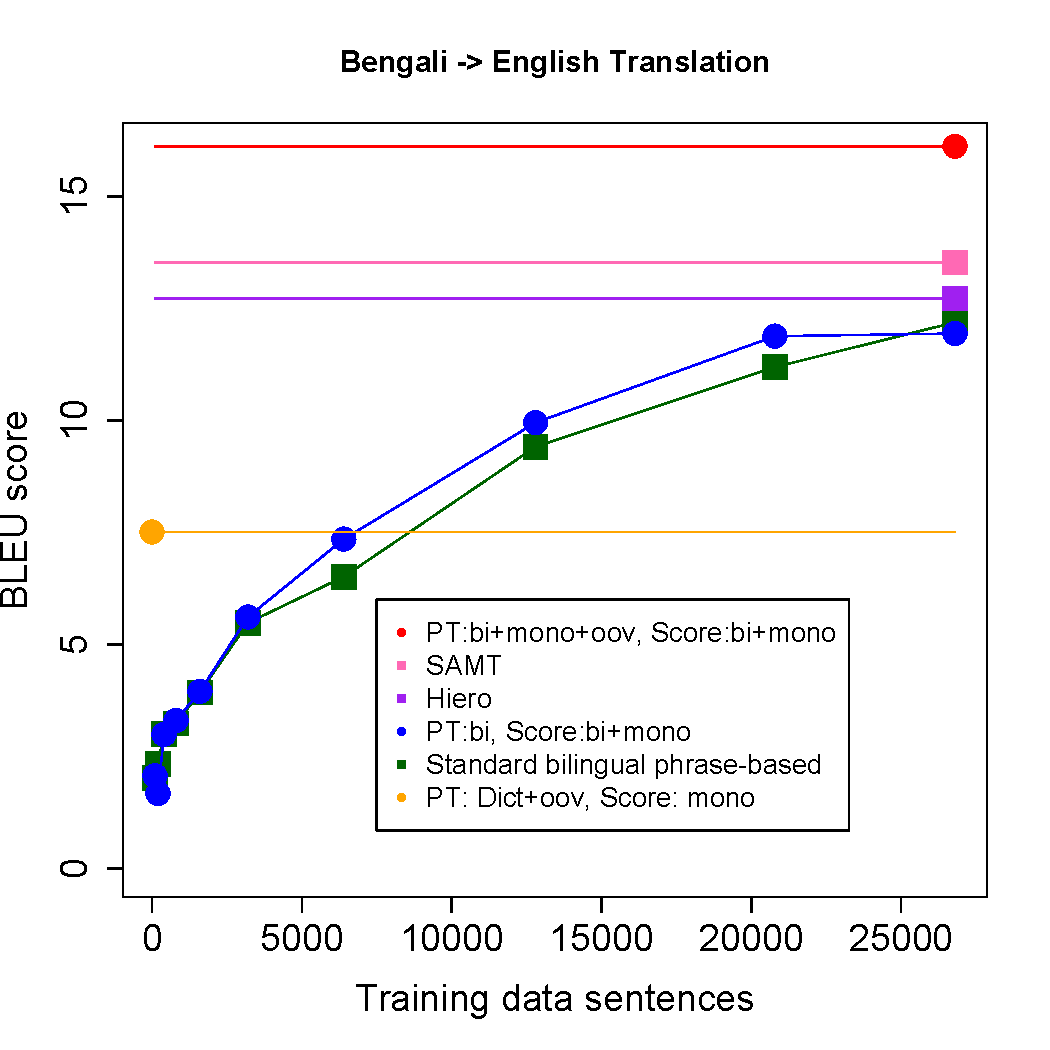
\includegraphics[width=1.05 \linewidth]{Figures/bntranslate.pdf}
\vskip -0.15in
\caption{End-to-end machine translation results for Bengali to English translation. It's noteworthy that the red line, which corresponds to our phrase-based system that uses the full available training data, our dictionaries, induced OOV translations and both bilingual and monolingual features outperforms all other experimental results.}
\vskip -0.2in
\label{fig:bntrans} 
\end{center}
\end{figure}

Unfortunately, these encouraging results aren't consistent across our Tamil and Hindi experiments. Figure \ref{fig:tatrans} shows the Tamil to English results. Here, both the Hiero and SAMT-based experiments presented in \newcite{post-callisonburch-osborne:2012:WMT} outperform our full system, which uses our complete phrase table, with bilingually extracted phrase pairs and both bilingually and monolingually estimated features. Additionally, adding monolingual features doesn't seem to help performance. However, it is nice to note that using only our given and induced bilingual dictionaries and our monolingual feature set to translate is equivalent to translating with a PBMT system trained on about $16,000$ parallel sentences.

\begin{figure}
\vskip 0.0in
\begin{center}
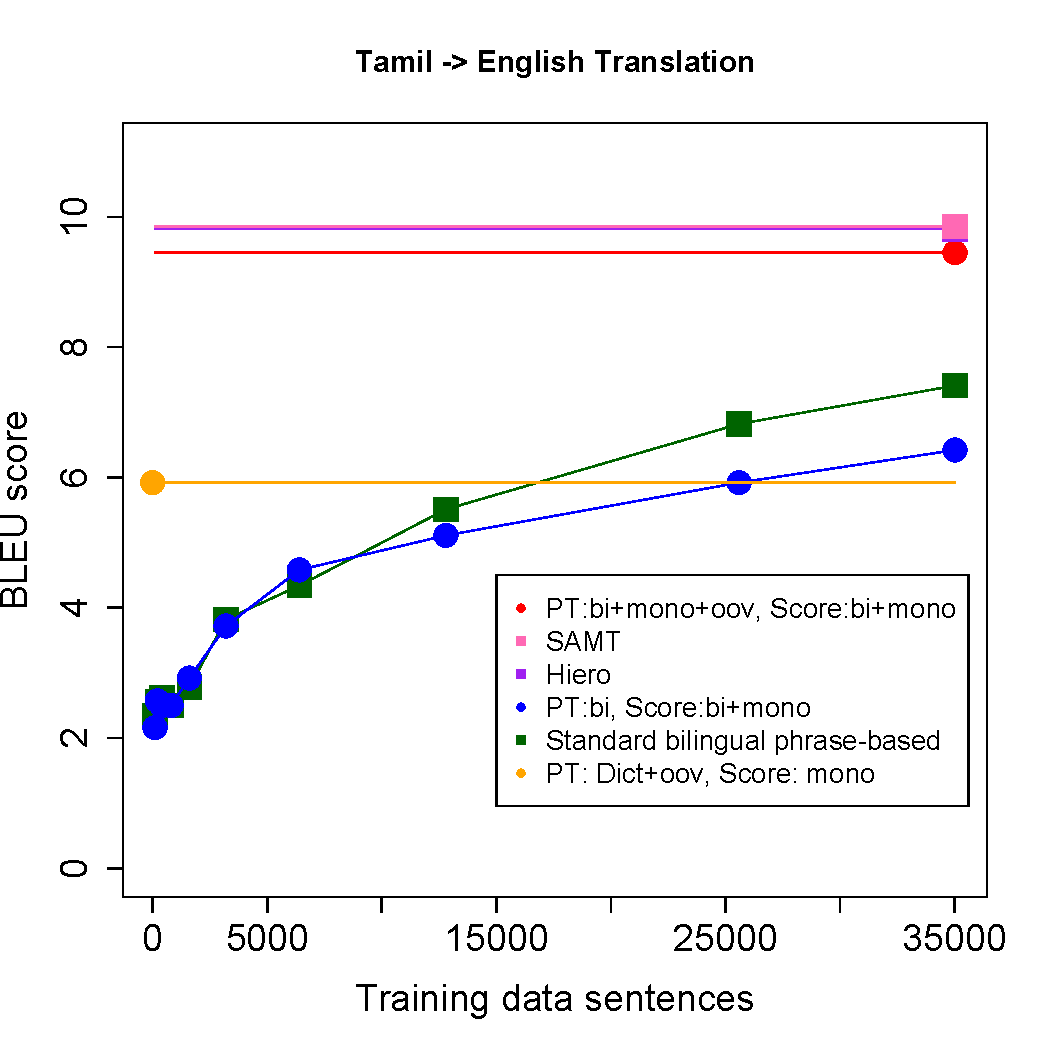
\includegraphics[width=1.05 \linewidth]{Figures/tatranslate.pdf}
\vskip -0.15in
\caption{End-to-end machine translation results for Tamil to English translation.}
\vskip -0.2in
\label{fig:tatrans} 
\end{center}
\end{figure}

\newpage

\bibliographystyle{naaclhlt2012}
\bibliography{bibliography}

\end{document}